\documentclass[11pt]{scrartcl}
\title{An Infrastructure to Store and Analyse Seismic Data as Suffix Trees}
\subtitle{MSc Data Analytics - Project Proposal}
\date{April 2016}
\author{Tom Taylor}

\usepackage[sort]{natbib}      % references
\usepackage[nottoc]{tocbibind} % bib om toc
\usepackage{hyperref}          % clickable links
\usepackage[all]{hypcap}       % for going to the top of an image when a figure reference is clicked
\usepackage{cleveref}

\usepackage{graphicx}
\graphicspath{ {img/} }
\setlength{\parindent}{4em}
\setlength{\parskip}{1em}

\begin{document}
\maketitle
\begin{itshape}
	\noindent This report is substantially the result of my own work except where explicitly indicated in the text. I give my permission for it to be submitted to the JISC Plagiarism Detection Service. I have read and understood the sections on plagiarism in the programme Handbook and the College website.
	
	\noindent The report may be freely copied and distributed provided the source is explicitly acknowledged.
\end{itshape}

\tableofcontents

\newpage

\section{Abstract}
	The purpose of this project is to develop an infrastructure and tool set for converting raw seismic time series data into a searchable string using SAX (\textbf{S}ymbolic \textbf{A}ggregate appro\textbf{X}imation) and then to store this data as a suffix tree for fast searching and analysis.  An interface will then be developed to enable the searching of these suffix trees and provide visualisation of the data.  This will enable the searching for similar patterns over time or between stations after an event.
	
	\noindent Potential applications of the software could be:
	\begin{itemize}
		\item Automatically finding the arrival times of events
		\item Correlating events across multiple stations
		\item Finding similar events at a given location at other times
	\end{itemize}
	
	The code should ideally be re-usable where possible in a project to receive live streaming data from many stations.
	
\section{Background}
\subsection{Seismic Waves}
	Seismic waves take on two main forms, body waves and surface waves.  Body waves are those that travel through the interior of the earth and are the fastest travelling.  The body waves are comprised of \textbf{P} (primary) waves which are compressional waves, travel fastest and thus arrive first.  \textbf{S} (secondary) waves are shear waves and travel more slowly, thus arrive later.  The separation between the phases is related to the distance of the earthquake and the local velocity structure. The surface waves travel only along the earth’s crust and, as they are confined to shallow depths where seismic velocities are slow, will normally arrive much later than the body waves.
	
	A seismic station records movement over three axis: vertical (\textbf{z}) alongside horizontal in terms of north-south (\textbf{n}) and east-west (\textbf{e}).  Due to seismic velocities generally increasing with depth, P waves arrive at a seismic station close to the vertical axis.  As a result, P waves can be measured as a simple metric of displacement along the Z axis.  S waves follow similar ray paths, but have their particle motion perpendicular to the direction of propagation.  As a result, they manifest on a seismogram as movement on both the n and e axis. The geometry of the fault tends to have a bearing on the orientation of the displacement so the two axis of movement cannot be easily combined in to a single metric for time series analysis.
	
\subsection{Symbolic Aggregate Approximation (SAX)}
	SAX (\textbf{S}ymbolic \textbf{A}ggregate appro\textbf{X}imation) \citep{sax} is a technique where by a single dimension of a time series is reduced to a string of symbols for pattern matching.  The technique involves first transforming the normalised time-series in to a Piecewise Aggregate Approximation (\textbf{PAA}) which is then represented by a fixed number of symbols.
	
	For the PAA, the data is first divided into equal sized time frames (see diagram below), then the mean deviation from zero of each frame is calculated.  An appropriate number of breakpoints symmetrical along the x-axis are created so that they follow a Gaussian distribution and a symbol assigned to each range between the breakpoints.  Then for each frame, a symbol is assigned based on which range the mean falls in to.  The symbols assigned to each frame are then concatenated in to a string and it is this string that gives the SAX representation of that data.  The width of the time frame and the number of discrete regions would be two parameters passed to this process alongside the data.
	\begin{figure}[h]
		\centering
		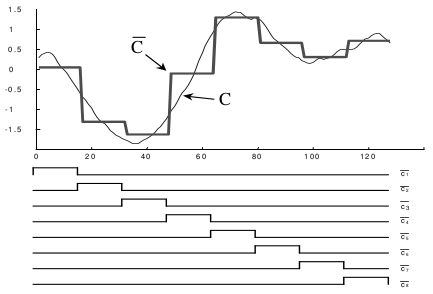
\includegraphics[scale=0.5]{paa.png}
		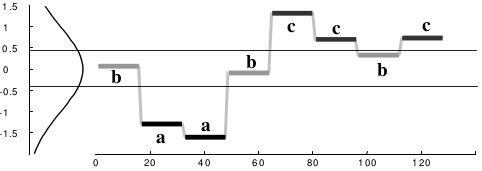
\includegraphics[scale=0.5]{sax.png}
		\caption{Diagrams showing PAA to SAX on a time-series (taken from \cite{sax})}
	\end{figure}
	
\subsection{Suffix Trees and the related infrastructure at Birkbeck}
	Suffix trees \citep{suffix} are a representation of a string designed for performing search related algorithms.  They are based on a suffix trie of a given string \textbf{T}.  The trie is constructed using all of the suffixes of \textbf{T} with a terminator character not used in the alphabet appended to the end of \textbf{T}.  The terminator is deemed to be lexicographically of lower priority than all of the other characters to ensure that a prefix of a string would appear before that string (such as in \textit{as} before \textit{ash}).  In the following example, the suffixes of \textit{T: abaaba} would produce the following suffixes with \textbf{\$} applied as a terminator.
	\begin{figure}[h]
		\centering
		\includegraphics[scale=0.5]{suffix_trie.png}
		\caption{Example Suffix Trie}
	\end{figure}
	
	This allows for efficient searching and counting substrings of \textbf{T} by following the trie from the root node.  Each substring \textbf{S} of \textbf{T} is a prefix of a path starting at the root.  It also allows for counting occurrences of the substring by finding the number of leaf nodes that can be reached from the end of the substring.  This format is not particularly space efficient as it has an upper bound storage in the order of \textit{$O(n^{2})$}.
	
	A far more efficient way to store and query the trie is to store it as Suffix Trees.  In order to produce a suffix tree from a trie, the non-branching nodes are firstly reduced (or coalesced) in to a single edge.  The original string \textbf{T} is then stored along side the tree and the labels further reduced to a starting position and offset within \textbf{T}.  The leaf nodes become labels to the offset of the suffix in the string.  This reduces the upper bound storage to \textit{$O(n)$} and results in a tree for our example \textbf{T} as seen in \cref{fig:tree}.
	\begin{figure}[h]
		\label{fig:tree}
		\centering
		\includegraphics[scale=0.5]{suffix_tree.png}
		\caption{Example Suffix Tree (edges shown as text and as positions/offsets)}
	\end{figure}
	
	This technique of building the tree is considered naive though as it is again very inefficient (being computationally in the order of \textit{$O(n^{3})$}).  It is far more desirable to achieve time-linear \textit{O(n)} construction of the tree.  An example of this is the Ukkonens Algorithm \citep{ukkonens}.  The algorithm is too long for inclusion but effectively starts with the implicit suffix tree of a string of length 1 and conditionally extends the tree on each iteration of adding a character.
	
	At Birkbeck, an infrastructure has been developed to load and query Suffix Trees \citep{bbk-suffix}.  At a high level it is based on language models but should be extendable to time series by the use of SAX.  There is current work in progress to utilise external memory (in this case Solid State Drives) to back the loaded Suffix Trees.  This would massively increase the maximum size of a tree to be queryable.  The current libraries to utilise this are written in Python however there is currently a refactor happening to C due to Python not being particularly computationally efficient because of its interpreted nature.  The trees in this implementation are stored as k-truncated trees for practical reasons.

\section{Objectives}
\begin{enumerate}
	\item Interpretation of raw data from seismic stations (in either the SAC or miniseed format) and storage as time-series data in a time-series database.
	\item Conversion of the time series data to SAX.
	\item Storage and querying of the SAX representation as a loadable suffix tree using the existing infrastructure.
	\item An interface for searching by SAX using Suffix trees and viewing the raw data.
\end{enumerate}

\section{Approach}
	As laid out in the objectives, the development will produce four separate components.
	
\subsection{Interpretation and Storage as time-series data}
	The raw data received from the stations is accessed as files in the SAC (Seismic Analysis Code) or miniseed binary formats.  These will be read using the ObsPy python library which can return both the headers and the raw data as a Python object.  Due to the complexities in analysing S waves (section 2.1), the scope of the project will be initially limited for searching for P waves on the Z axis only.  However the interface will still have access to the raw data for all three axis and be able to show all three together for analysis by a seismologist.
	
	This data will be batch processed and imported in to a time series database.  Initially OpenTSDB is being considered for performance reasons but there may be scope for this to change depending on how difficult it is to implement this on the Universities hardware.  Other options could be InfluxDB or Graphite which are considerably easier to implement but might suffer from scalability issues.

\subsection{Conversion of data to SAX}
	Once the raw data has been loaded to the time series database, it will be re-read in batches and passed though an algorithm to produce a SAX string (as described in section 2.2).  There are a few challenges in making this string usable.  Firstly the seismic data will need to have noise removed and to be normalised across multiple stations.  Secondly the parameters of alphabet length and the size of the time window most suitable will need to be empirically found.  The SAX implementation itself should be generic so that it can be used for other time series data.
	
\subsection{Storage as a Suffix Tree}
	Once a suitable SAX string can be created across the dataset, it will be loaded in to a suffix tree using the toolset and infrastructure available at Birkbeck.  The methodology will ultimately be influenced by the exposed API once the aforementioned refactor is complete.

\subsection{Interface to query the data}
	The interface to query and view the data will be web based so as to ensure maximum compatibility with clients.  Many open source graph renderers are in existence such as (Grafana and Cubism.js) and components of both are likely to be used for viewing the raw seismic data alongside the SAX data.

\section{Plan}
	The various components (parsing, SAX, interface to the Suffix Tree infrastructure, Graphical Interface, etc.) will all be written separately and act as micro services.  They will each be callable via a REST HTTP API to reduce any compatibility issues between any technologies used and to increase portability for use in other projects.

	Much of the coding is planned to be done in Python 3.  This is because the working prototype for the Suffix Tree infrastructure at Birkbeck is currently written in Python.  Also the Python library ObsPy is considered relatively mature and has been shown to work with the raw sample data.
	
	One potential limitation for using Python is the multi-threading components (for the cPython implementation at least) as it relies on the concept of a Global Interpreter Lock.  The GIL effectively prevents multiple threads from running simultaneously to avoid potentially non-thread-safe operations from conflicting with each other.  This will very likely have an impact on the speed of data analysis when working over large datasets so other languages may be considered.  Also the maturity of various libraries will be considered when making language choices over individual components.  Other languages that might come in to play to overcome this shortcoming are R and Scala.
	
	Development will take the approach of Test Driven Development (TDD) where functional tests and class level unit tests will be written for each component and the test suite will be used within the build environment during development.
	
	For training and initial validation of the effectiveness of the software, some sample data based on research at the Nabro volcano in Eritrea during 2011 \citep{eritrea1}, \citep{eritrea2} will be provided by the Department of Earth and Planetary Sciences at Birkbeck.  Key events have already been manually picked from this data.  Further data will then be provided for test set validation.
	
	Once a proof of concept is functioning, work will again be coordinated with the Department of Earth and Planetary Sciences to find suitable parameters for the normalisation of the seismic data and for the time frame and alphabet sizes for the SAX implementation.
	
	Where possible, alternative implementations of the data intensive tasks will also be compared and benchmarked for performance and accuracy.

\bibliographystyle{humannat}
\bibliography{bibliography}

\end{document}
